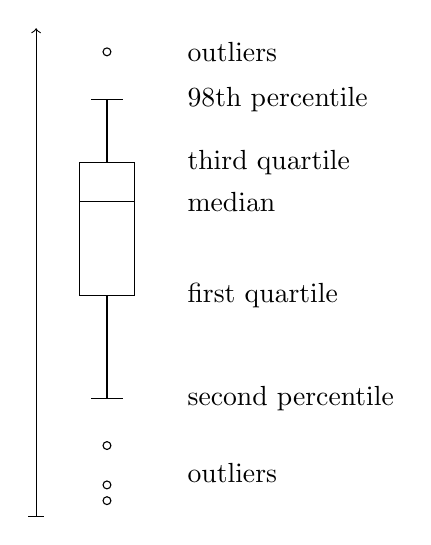
\begin{tikzpicture}[]

\def \xmid{0.9cm}
\def \xtext{1.8cm}
\def \boxwidth{0.7cm}
\def \whiskerwidth{0.4cm}

\def \youtlierbelowa{0.2cm}
\def \youtlierbelowb{0.4cm}
\def \youtlierbelowc{0.9cm}
\def \youtlierabove{5.9cm}

\def \ysec{1.5cm} % 2nd percentile
\def \yfir{2.8cm} % 1st quartile
\def \ymed{4.0cm} % median
\def \ythi{4.5cm} % 3rd quartile
\def \ynin{5.3cm} % 98th percentile

% y axis
\draw[->] (0cm , 0cm) -- (0cm, 6.2cm);
\draw[-] (-0.1cm, 0cm) -- (0.1cm, 0cm);

% hor lines from bottom to top
\draw[-] (\xmid - \whiskerwidth/2, \ysec) -- (\xmid + \whiskerwidth/2, \ysec);
\draw[-] (\xmid - \boxwidth    /2, \yfir) -- (\xmid + \boxwidth    /2, \yfir);
\draw[-] (\xmid - \boxwidth    /2, \ymed) -- (\xmid + \boxwidth    /2, \ymed);
\draw[-] (\xmid - \boxwidth    /2, \ythi) -- (\xmid + \boxwidth    /2, \ythi);
\draw[-] (\xmid - \whiskerwidth/2, \ynin) -- (\xmid + \whiskerwidth/2, \ynin);

% vert lines from bottom to top and left to right
\draw[-] (\xmid                  , \ysec) -- (\xmid              , \yfir);
\draw[-] (\xmid - \boxwidth    /2, \yfir) -- (\xmid - \boxwidth/2, \ythi);
\draw[-] (\xmid + \boxwidth    /2, \yfir) -- (\xmid + \boxwidth/2, \ythi);
\draw[-] (\xmid                  , \ythi) -- (\xmid              , \ynin);

% outliers from bottom to top
\node[draw, circle, inner sep=0pt, minimum size=0.1cm] at (\xmid, \youtlierbelowa) {};
\node[draw, circle, inner sep=0pt, minimum size=0.1cm] at (\xmid, \youtlierbelowb) {};
\node[draw, circle, inner sep=0pt, minimum size=0.1cm] at (\xmid, \youtlierbelowc) {};
\node[draw, circle, inner sep=0pt, minimum size=0.1cm] at (\xmid, \youtlierabove)  {};

% text from bottom to top
\node[draw=none, anchor=west] at (\xtext, \youtlierbelowa/2 + \youtlierbelowc/2) {outliers};
\node[draw=none, anchor=west] at (\xtext, \ysec)          {second percentile};
\node[draw=none, anchor=west] at (\xtext, \yfir)          {first quartile};
\node[draw=none, anchor=west] at (\xtext, \ymed)          {median};
\node[draw=none, anchor=west] at (\xtext, \ythi)          {third quartile};
\node[draw=none, anchor=west] at (\xtext, \ynin)          {98th percentile};
\node[draw=none, anchor=west] at (\xtext, \youtlierabove) {outliers};

\end{tikzpicture}
